\section{Stateful Session Beans}
\label{sec:chap2:sfsb}

Eine Stateful Session Bean ist ein EJB das seinen internen Status "uber mehrere Aufrufe hinweg beibehalten kann.
Methodenaufrufe des Client an einem bestimmten Stub werden immer an die selbe Bean-Instanz weitergeleitet, somit
behalten alle Felder der Bean ihre Werte solange der Client den Stub h"alt.
\begin{floatingfigure}[!h]{80mm}
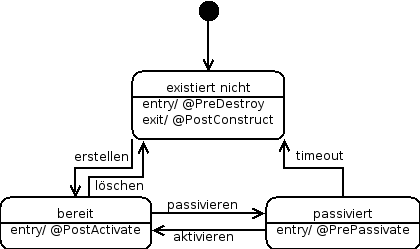
\includegraphics[width=75mm]{chap2/img/sfsbstates.png}
\caption{Lebenszyklus einer Stateful Session Bean, mit Annotationen}
\label{fig:sfsbstates}
\end{floatingfigure}
Zwar geschieht das Erstellen, Vorhalten und L"oschen der einzelnen Bean-Instanzen vollautomatisch durch den EJB-Container, 
trotzdem besteht manchmal die Notwendigkeit den Lebenszyklus einer Bean zu beeinflussen. Hierf"ur mussten in fr"uheren
EJB-Versionen sogenannte "'Lifecycle-Callbacks"' implementiert werden. In EJB 3.0 sind diese Callbacks "uberfl"ussig,
und werden durch spezielle Annotationen ersetzt, die zu bestimmten Zeitpunkten im Lebenszyklus aufzurufende Methoden
vermerken. Abbildung \ref{fig:sfsbstates} stellt den Lebenszyklus einer Stateful Session Bean zusammen mit den jeweiligen
Annotationen dar.
Die meisten dieser Annotationen sind sowohl f"ur Stateful, als auch f"ur Stateless Session Beans zul"assig,
im folgenden sollen die wichtigsten aufgef"uhrt werden:
\begin{description}
\item[@PostConstruct]
Die annotierte Methode wird direkt nachdem die Instanz erstellt wurde vom Container aufgerufen, @PostConstruct ist sowohl
f"ur Stateful als auch f"ur Stateless Session Beans zul"assig.
\item[@PreDestroy]
Die annotierte Methode wird aufgerufen bevor der Container eine unbenutzte oder ausgelaufene Instanz aus seinem Objektpool
l"oscht, @PreDestroy ist sowohl f"ur Stateful als auch f"ur Stateless Session Beans zul"assig.
\item[@PrePassivate]
Wenn eine Stateful Session Beans Instanz zu lange nicht aufgerufen wird kann der Container diese passivieren, und ihren
Zustand in seinem Cache zwischenspeichern. Eine mit @PrePassivate annotierte Methode wird direkt vor dem Passivieren aufgerufen.
\item[@PostActivate]
Wenn eine Anfrage an eine passivierte Bean gestellt wird wird eine neue Instanz der Bean-Klasse erzeugt und der vormalige
Zustand wieder hergestellt. Nachdem dies geschehen ist, aber bevor der Aufruf schliesslich an die Bean-Instanz weitergeleitet
wird wird die mit @PostActivate annotierte Methode aufgerufen. Diese Annotation ist nur f"ur Stateful Session Beans zul"assig.
\item[@Init]
Diese Annotation bezeichnet Initialisierungsmethoden f"ur eine Stateful Session Beans. Der Unterschied zu @PostConstruct
besteht darin, dass innerhalb einer Bean-Klasse mehrere Methoden mit @Init annotiert werden k"onnen, allerdings wird immer nur
eine dieser Methoden tats"achlich vom Container aufgerufen. Welche das ist bestimmt sich aus der Art und Weise, wie die
Bean erstellt wurde, n"aheres ist der EJB 3.0 \cite{EJBHP} zu entnehmen. Die @Init-Methode wird noch vor der 
@PostConstruct-Methode aufgerufen.
\end{description}


\subsection{Interface}
\label{sec:chap2:sfsb:if}

Um die zustandsvorhaltenden Eigenschaften der Stateful Session Bean zu testen enth"alt das Service-Interface eine Methode 
um den Namen der zu gr"u\ss enden Person zu setzen. Die Gru\ss methode selbst nimmt folglich keine Parameter entgegen, sondern
nutzt den zuvor gesetzten Namen um die Gru\ss botschaft zu erstellen.
\begin{lstlisting}[caption=Stateful Hello World Interface]
public interface SFHelloWorld {
    public void setName(String s) throws ScriptException;
    public String sayHello() throws ScriptException;
}
\end{lstlisting}

\subsection{PHP-Implementation}
\label{sec:chap2:sfsb:impl}

Im Gegensatz zum Service-Interface unterscheidet sich die Implementierung der Stateful Session Bean erheblich von der
Stateless Session Bean. Da der Zustand der Bean nicht im Java-Teil, sondern vom PHP-Code vorgehalten werden sollte
mussten Lebenszyklus-Methoden implementiert werden.

Zun"achst wurde die mit \emph{@PostConstruct} annotierte Methode \emph{initialize()} geschrieben, in der der Quelltext
"ubersetzt und eine Instanz der implementierenden PHP-Klasse erzeugt wird. Dieses Erzeugen geschieht mittels einer
Art "'friend-Methode"', aber es sind auch beliebige andere Methoden denkbar.
Sowohl das "ubersetzte Skript als auch das PHPObject der PHP-Klasse werden als Attribute der Bean gespeichert. 
Allerdings konnten diese Attribute aus zwei
Gr"unden nicht zur Speicherung des Zustandes genutzt werden: zum einen sollte im Hinblick auf eine m"ogliche
Automatisierung s"amtliche Funktionalit"at in PHP realisiert werden, und zum anderen kann innerhalb des Bean-Containers
nicht davon ausgegangen werden, dass die in ByteBuffern gespeicherten Informationen - der Zend-Opcode des "ubersetzten
Skriptes und vor allem der C-Pointer auf den Zval des PHP-Objektes - beim n"achsten Aufruf einer Bean-Methode noch valide 
sind. Folglich mussten der Bean zwei weitere Methoden hinzugef"ugt werden, die mit \emph{@PrePassivate} annotierte Methode
\emph{sleep()}, und die mit \emph{@PostActivate} annotierte Methode \emph{wakeUp()}. Als Methode zur Persistierung des
PHP-Objektes wurde der PHP-Mechanismus zur Serialisierung von Daten gew"ahlt, hierzu wurden der PHP-Klasse die Methoden
\emph{ser()} und \emph{unser()} hinzugef"ugt, erstere gibt einen String zur"uck der eine serialisierte Fassung des Objektes
enth"alt, letztere nimmt einen solchen String entgegen und stellt daraus den urspr"unglichen Zustand wieder her.
Damit gew"ahrleistet ist dass die oben angesprochenen Attribute der Java-Klasse nicht versehentlich persistiert werden 
werden die Referenzen der beiden Objekte auf null gesetzt.
Die Aufrufe der eigentlichen Service-Methoden werden genau wie bei der Stateless Session Bean mittels des Invocable-Interfaces
durchgef"uhrt, ihr Implementation in PHP gestaltete sich als trivial
\begin{lstlisting}[caption=PHP-Implementierung]
<?php
class SFHelloWorld {
  var $name = 'initial value';
  function setName($n) {
    $this->name = $n;
  }
  function sayHello() {
    return 'Stateful PHP says hello to '.$this->name;
  }
  function ser($obj) {
    return serialize($obj);
  }
  function unser($str) {
    $cpy = unserialize($str);
    $this->setName($cpy->name);
  }
}
\end{lstlisting}


